\documentclass[accentcolor=tud1d,colorbacktitle,inverttitle,landscape,german,presentation,t]{tudbeamer}
\usepackage[latin1]{inputenc}
\usepackage[english]{babel}
\usepackage{amsmath}
\usepackage{amsfonts}
\usepackage{amssymb}
\usepackage{graphicx}
\usepackage{natbib}

\usepackage{algorithm}
\usepackage{algorithmic}

\newcommand{\x}{\item}
\newcommand{\parTitle}[1]{\textbf{#1:}}
\DeclareMathOperator{\E}{\mathbb{E}}
\setlength\parindent{0pt}

\begin{document}
	
	\title[Natural Actor Critic]{Natural Actor Critic \\Components and Extensions}
	\subtitle{Maximilian Gehrke\\Tabea Wilke\\Yannik Frisch\\\\Group 19 Oleg 
	Arenz}
	
	\author[Maximilian Gehrke et al.]{Tabea Wilke, Yannik Frisch and Maximilial 
	Gehrke}
	\institute[IAS TU Darmstadt | Group 19]{Institute for Intelligent Autonomous Systems, TU Darmstadt}
	
	
	\logo{
\includegraphics{iasLogo}}
	%\logo{\color{tudtextaccent}\large IFP}
	
	\date{March 22, 2019}
	

\begin{titleframe}
\end{titleframe}
\section{Introduction}
	\begin{frame}
		\frametitle{\\Natural Gradient}
		
		\begin{itemize}		
			\x Optimization problem:
			\begin{align*}
				\max_{\delta\theta} J(\theta + \delta\theta) \approx J(\theta) + \delta\theta^T\nabla_\theta J(\theta)\\
				\text{s.t. } \epsilon = D_{KL}(\pi_{\theta} ||�\pi_{\theta + \delta\theta}) \approx \tfrac{1}{2} \delta\theta^T F_\theta \delta\theta
			\end{align*}
			\x Solution:
			\begin{equation*}
				\widetilde{\nabla}_{\theta} J(\theta) = F_\theta^{-1} \nabla_\theta J(\theta)
			\end{equation*}
			\x Fisher Information Matrix:
			\begin{equation*}
					F_\theta=\E_{\pi_\theta}\left[\nabla_{\theta}\log\pi_{\theta}(a|s)\nabla_{\theta}\log\pi_{\theta}(a|s)^{T}\right]
			\end{equation*}
		\end{itemize}
		\vspace{3mm}
		\hspace{3mm}$\Rightarrow$\hspace{7mm} \textit{Parametrization invariant, data efficient \& fast convergence}
	\end{frame}
	\begin{frame}
		\frametitle{\\The Natural Actor Critic algorithm}
		\centering
		\vspace{-3.5mm}
		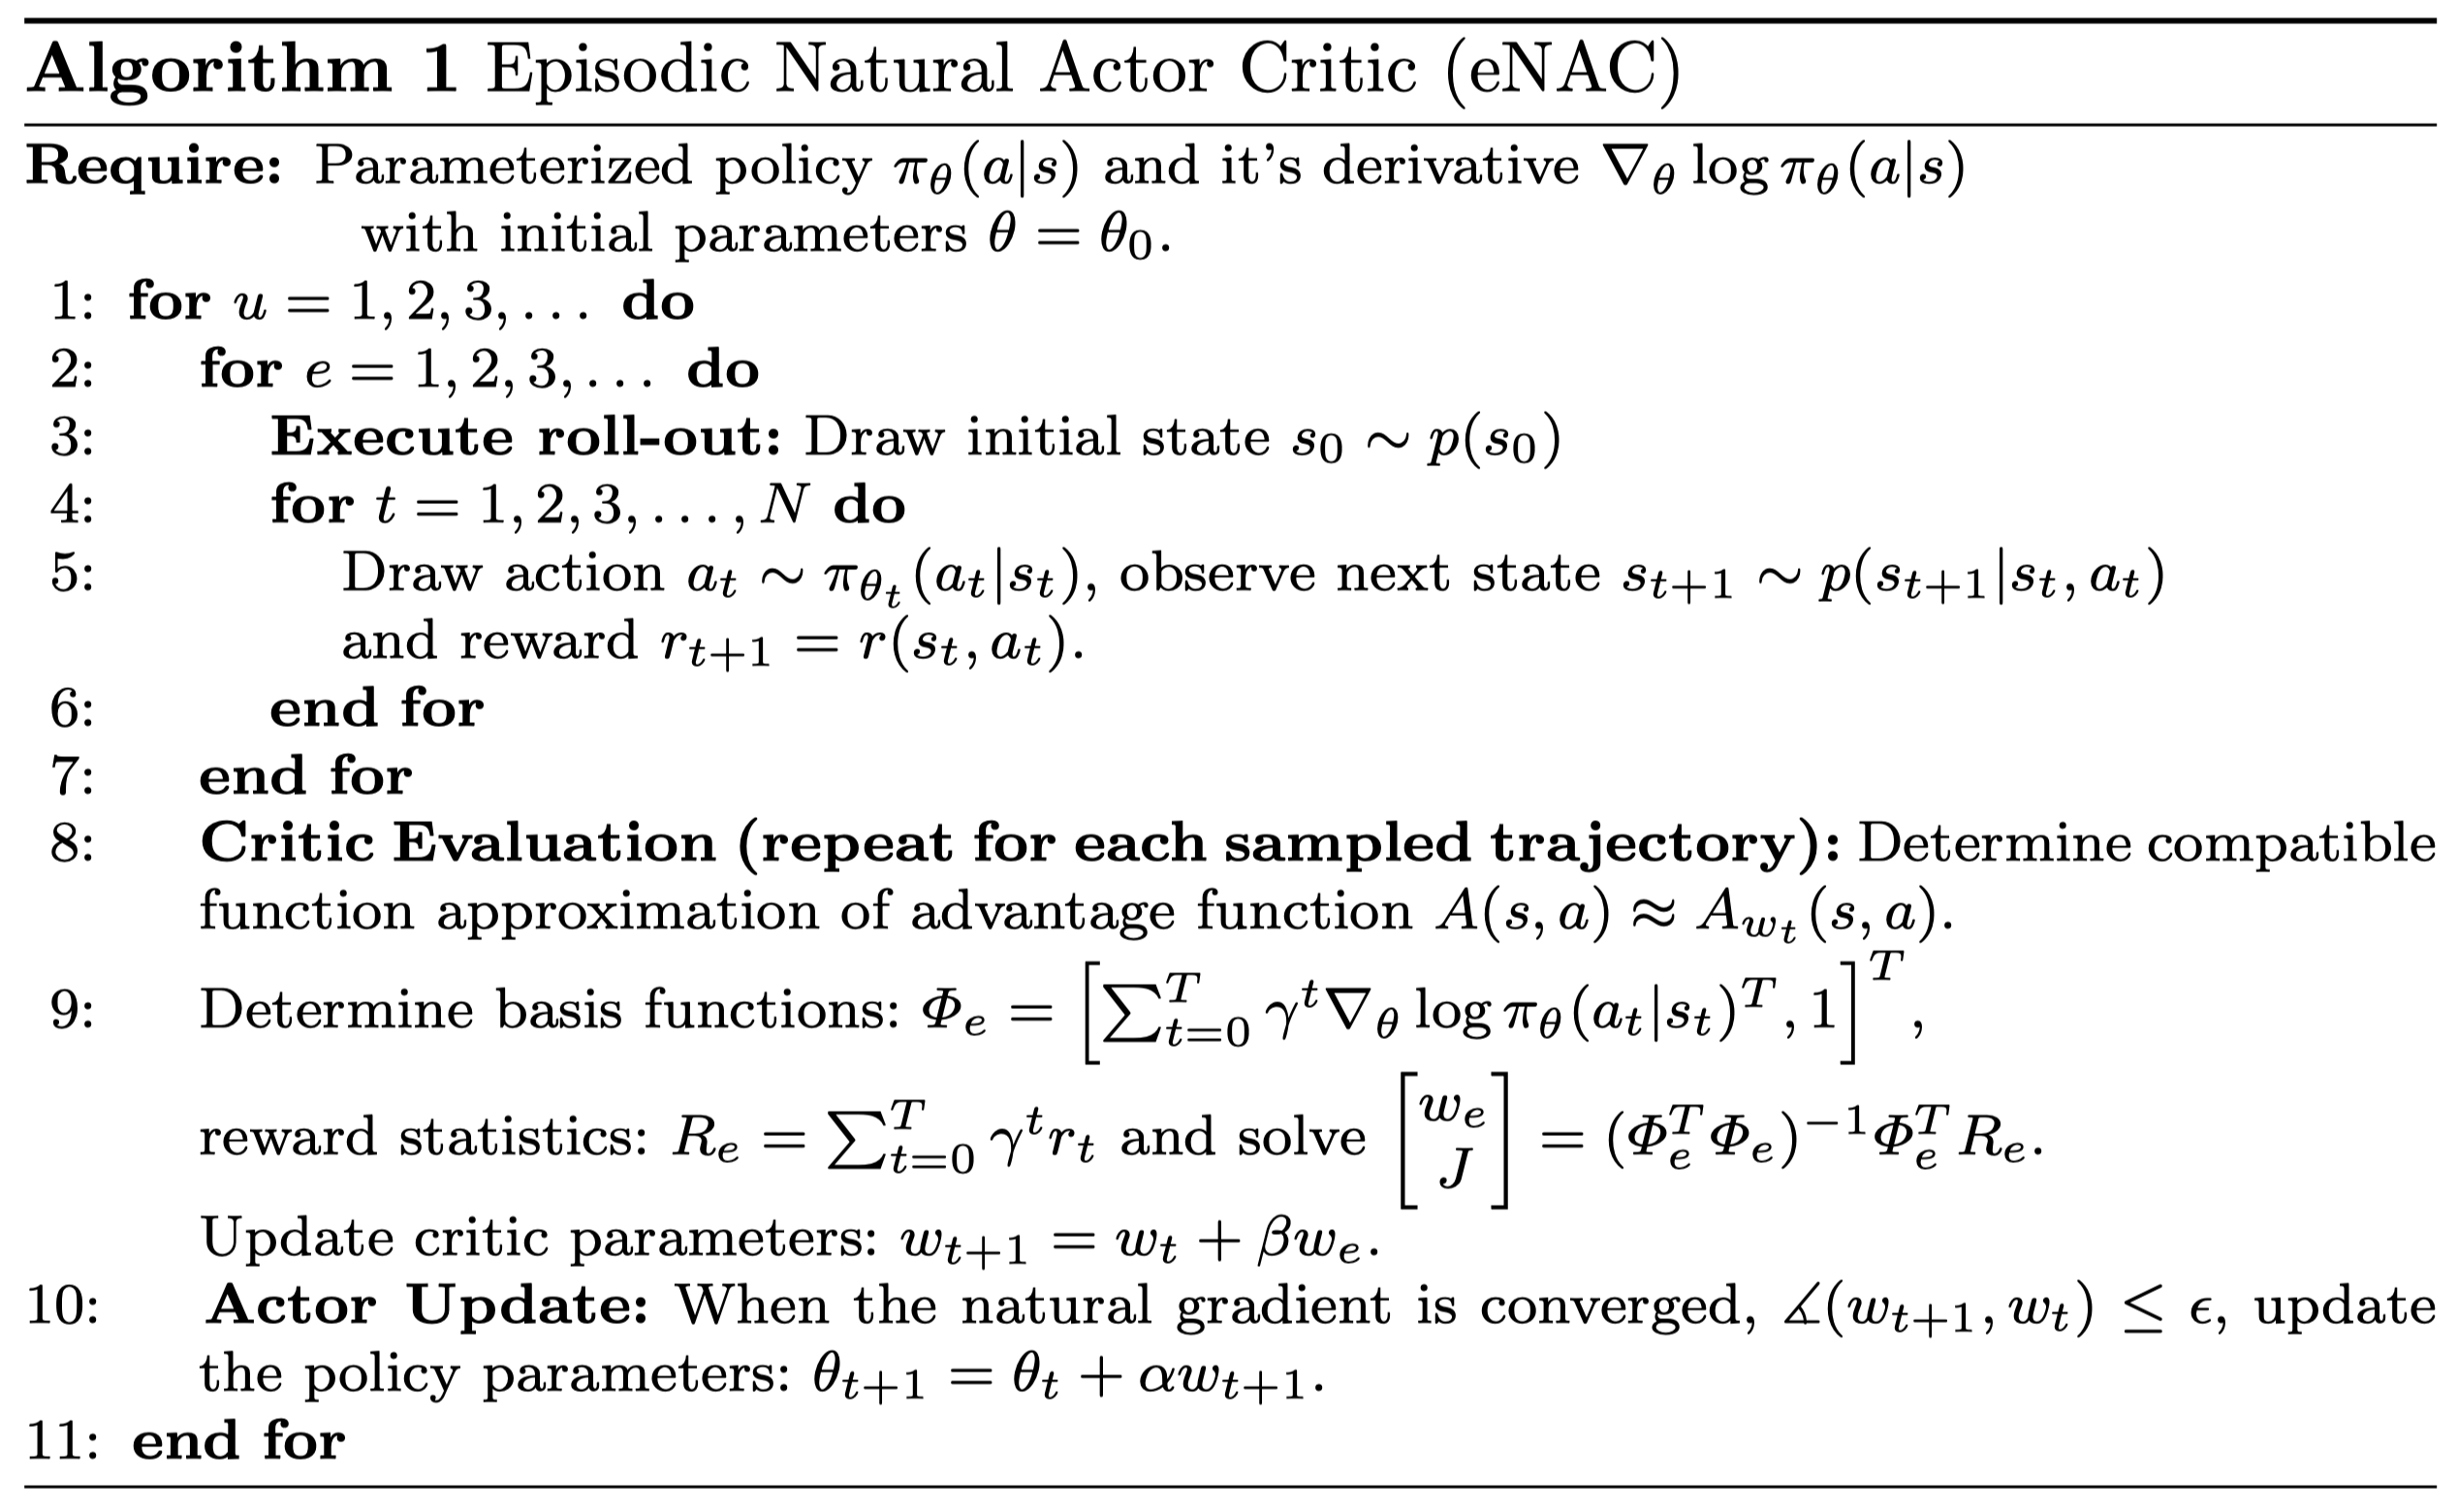
\includegraphics[scale=0.24]{nac_algorithm.png}
	\end{frame}

	\begin{frame}
		\frametitle{\\Extensions}
		\begin{itemize}
			\x Recursive Least Squares
			\vspace{1mm}
			\x Fitted NAC + Importance Sampling (FNAC)			\vspace{1mm}
			\x Incremental NAC (INAC)			\vspace{1mm}
			\x Implicit Incremental NAC (I2NAC)			\vspace{1mm}
			\x Regularization
		\end{itemize}
	\end{frame}

	\begin{frame}
		\frametitle{\\Conclusion \& Discussion}
		\begin{itemize}
			\x NAC has several advantages over vanilla PGM
			\vspace{4mm}
			\x Different approaches for:
			\begin{itemize}
				\x Updating critic (\& adjusting learning rate)
				\x Fisher inverse
				\x Actor update frequency 
			\end{itemize}
		\vspace{4mm}
			\x Open Questions:
			\begin{itemize}
				\x Inverse of Fisher Information Matrix (expensive!)
				\x NPG estimation might be biased \citep{thomas2014bias}
				\x Application to POMDP's \citep{jurvcivcek2011natural}
			\end{itemize}
		\end{itemize}
	\end{frame}


	
	\begin{frame}
		\frametitle{\\Sources}
		For publication references please see our paper \textit{``Natural Actor Critic: Components and Extensions''}.
		
		\vspace{5mm}

		\bibliographystyle{dinat}
		\bibliography{Group19_nac_presentation.bib} 
		
	\end{frame}
	
\end{document}